
\chapter{Introduction\label{ch:intro}}

Our understanding of fundamental particles and interactions has progressed much from the early days.
These beginnings could be with Empdocles and his four roots fire, earth, air, and water, or with
Aristotle relating these four roots to two of the four sensible quantities hot, dry, wet, and
cold~\cite{0415078547} as in Figure~\ref{fig:aristotle}
(not to omit classical elements from other philosophies and worldviews), or more recently with
John Dalton's atoms~\cite{dalton}. Or perhaps particle physics began with
the discovery of the electron by J.J. Thomson in 1897~\cite{thomson:electron},
which to this day has not been observed
to have internal structure or decay, with upper (lower) bounds on the radius (lifetime) of
10$^{-22}$~m (10$^{26}$~years)~\cite{1988PhST...22..102D,2002PhLB..525...29B}.

\begin{figure}[ht]
 \begin{center}
    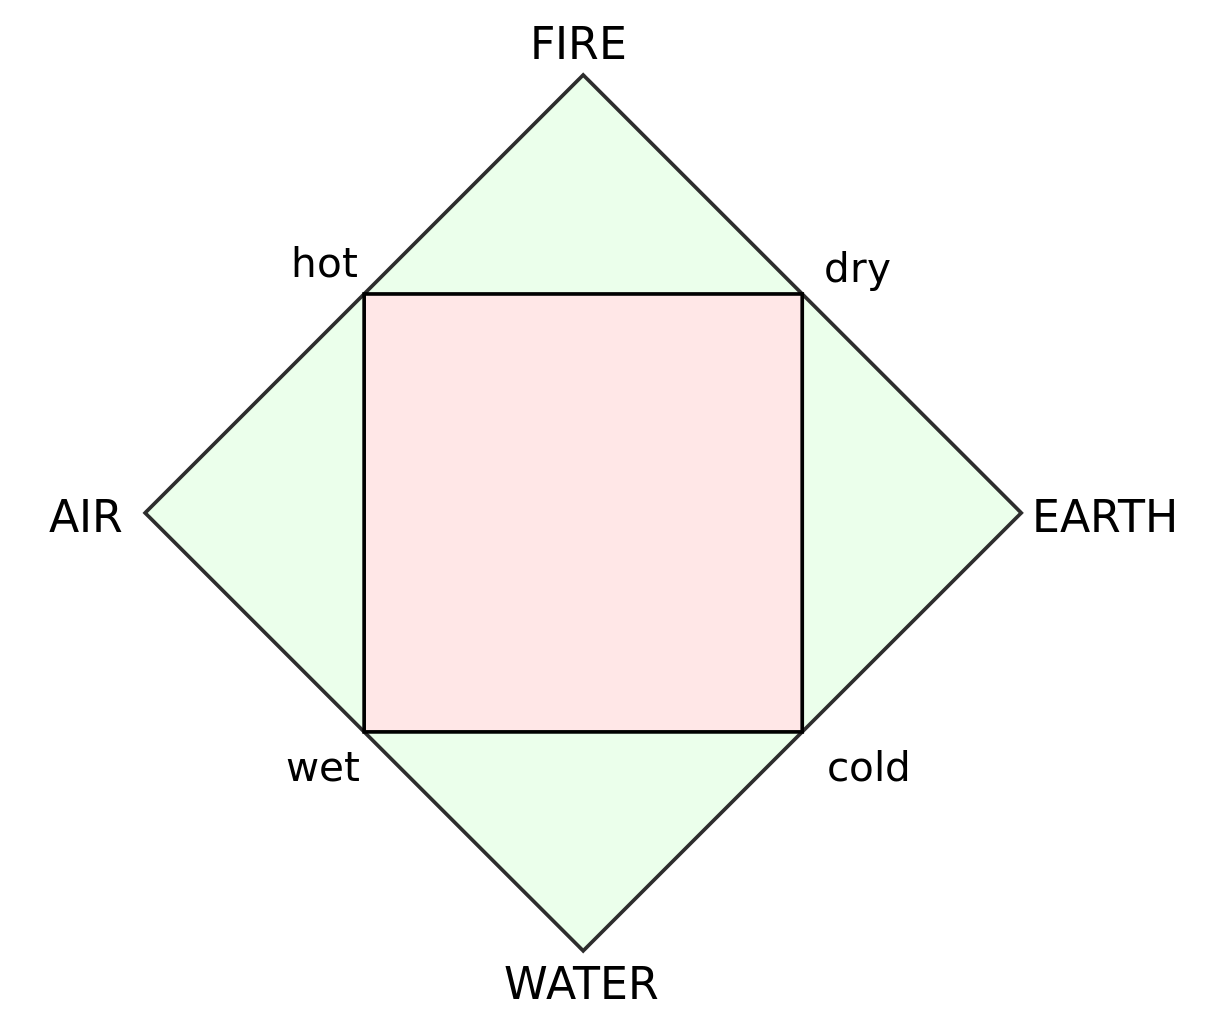
\includegraphics[width=0.50\textwidth]{figures/intro/Four_elements_representation.png}
      \end{center}
\caption{The four roots how they relate to the sensible quantities.}
\label{fig:aristotle}
\end{figure}

Today we have the Standard Model, the theoretical framework that best describes the
experimentally observed phenomena of the fundamental particles and their interactions. The theory
is not perfect, and it remains an overarching theme of particle physics to unify physical processes
at all energy scales under one single framework, if such a thing can be done at all.
The SM and its shortcomings are described in
Sections~\ref{sec:SM} and \ref{sec:SMshortcomings}.

Recently in 2012, the last piece to the SM was put into place with the discovery of the Higgs boson.
This discovery, described in Section~\ref{sec:discovery}, is the foundation for the work based on
this thesis, the goal of which is to describe the first search for double Higgs production, a process
in which two Higgs bosons are produced. The motivations for what the search for this process means
in the context of SM physics and ``new'' physics is given in Section~\ref{sec:diHiggs}.

Finally, for those readers who have by chance come across this thesis and do not
have any physics training, Appendix~\ref{ch:mom} may be especially appealing.

\section{The Standard Model\label{sec:SM}}

The Standard Model (SM) of particle physics is a relativistic quantum field theory
that describes how the known fundamental particles interact through the electromagnetic, weak,
and strong forces.
The theory was developed through the unification of the electromagnetic and weak forces by Glashow
in 1961~\cite{1961.Glashow.Partial-symmetries} and through the incorporation of this electroweak
theory with the Higgs mechanism by Weinberg and Salam in 1967~\cite{PhysRevLett.19.1264,Salam:1968rm}.
This theory explained the experimental observations of the day, and later experiments provided
additional evidence as well as a mean for measuring the free parameters of the theory. Some of
this evidence is provided in Figure~\ref{fig:discoveries} in the form of the discoveries of
the fundamental particles.

\begin{figure}[ht]
 \begin{center}
    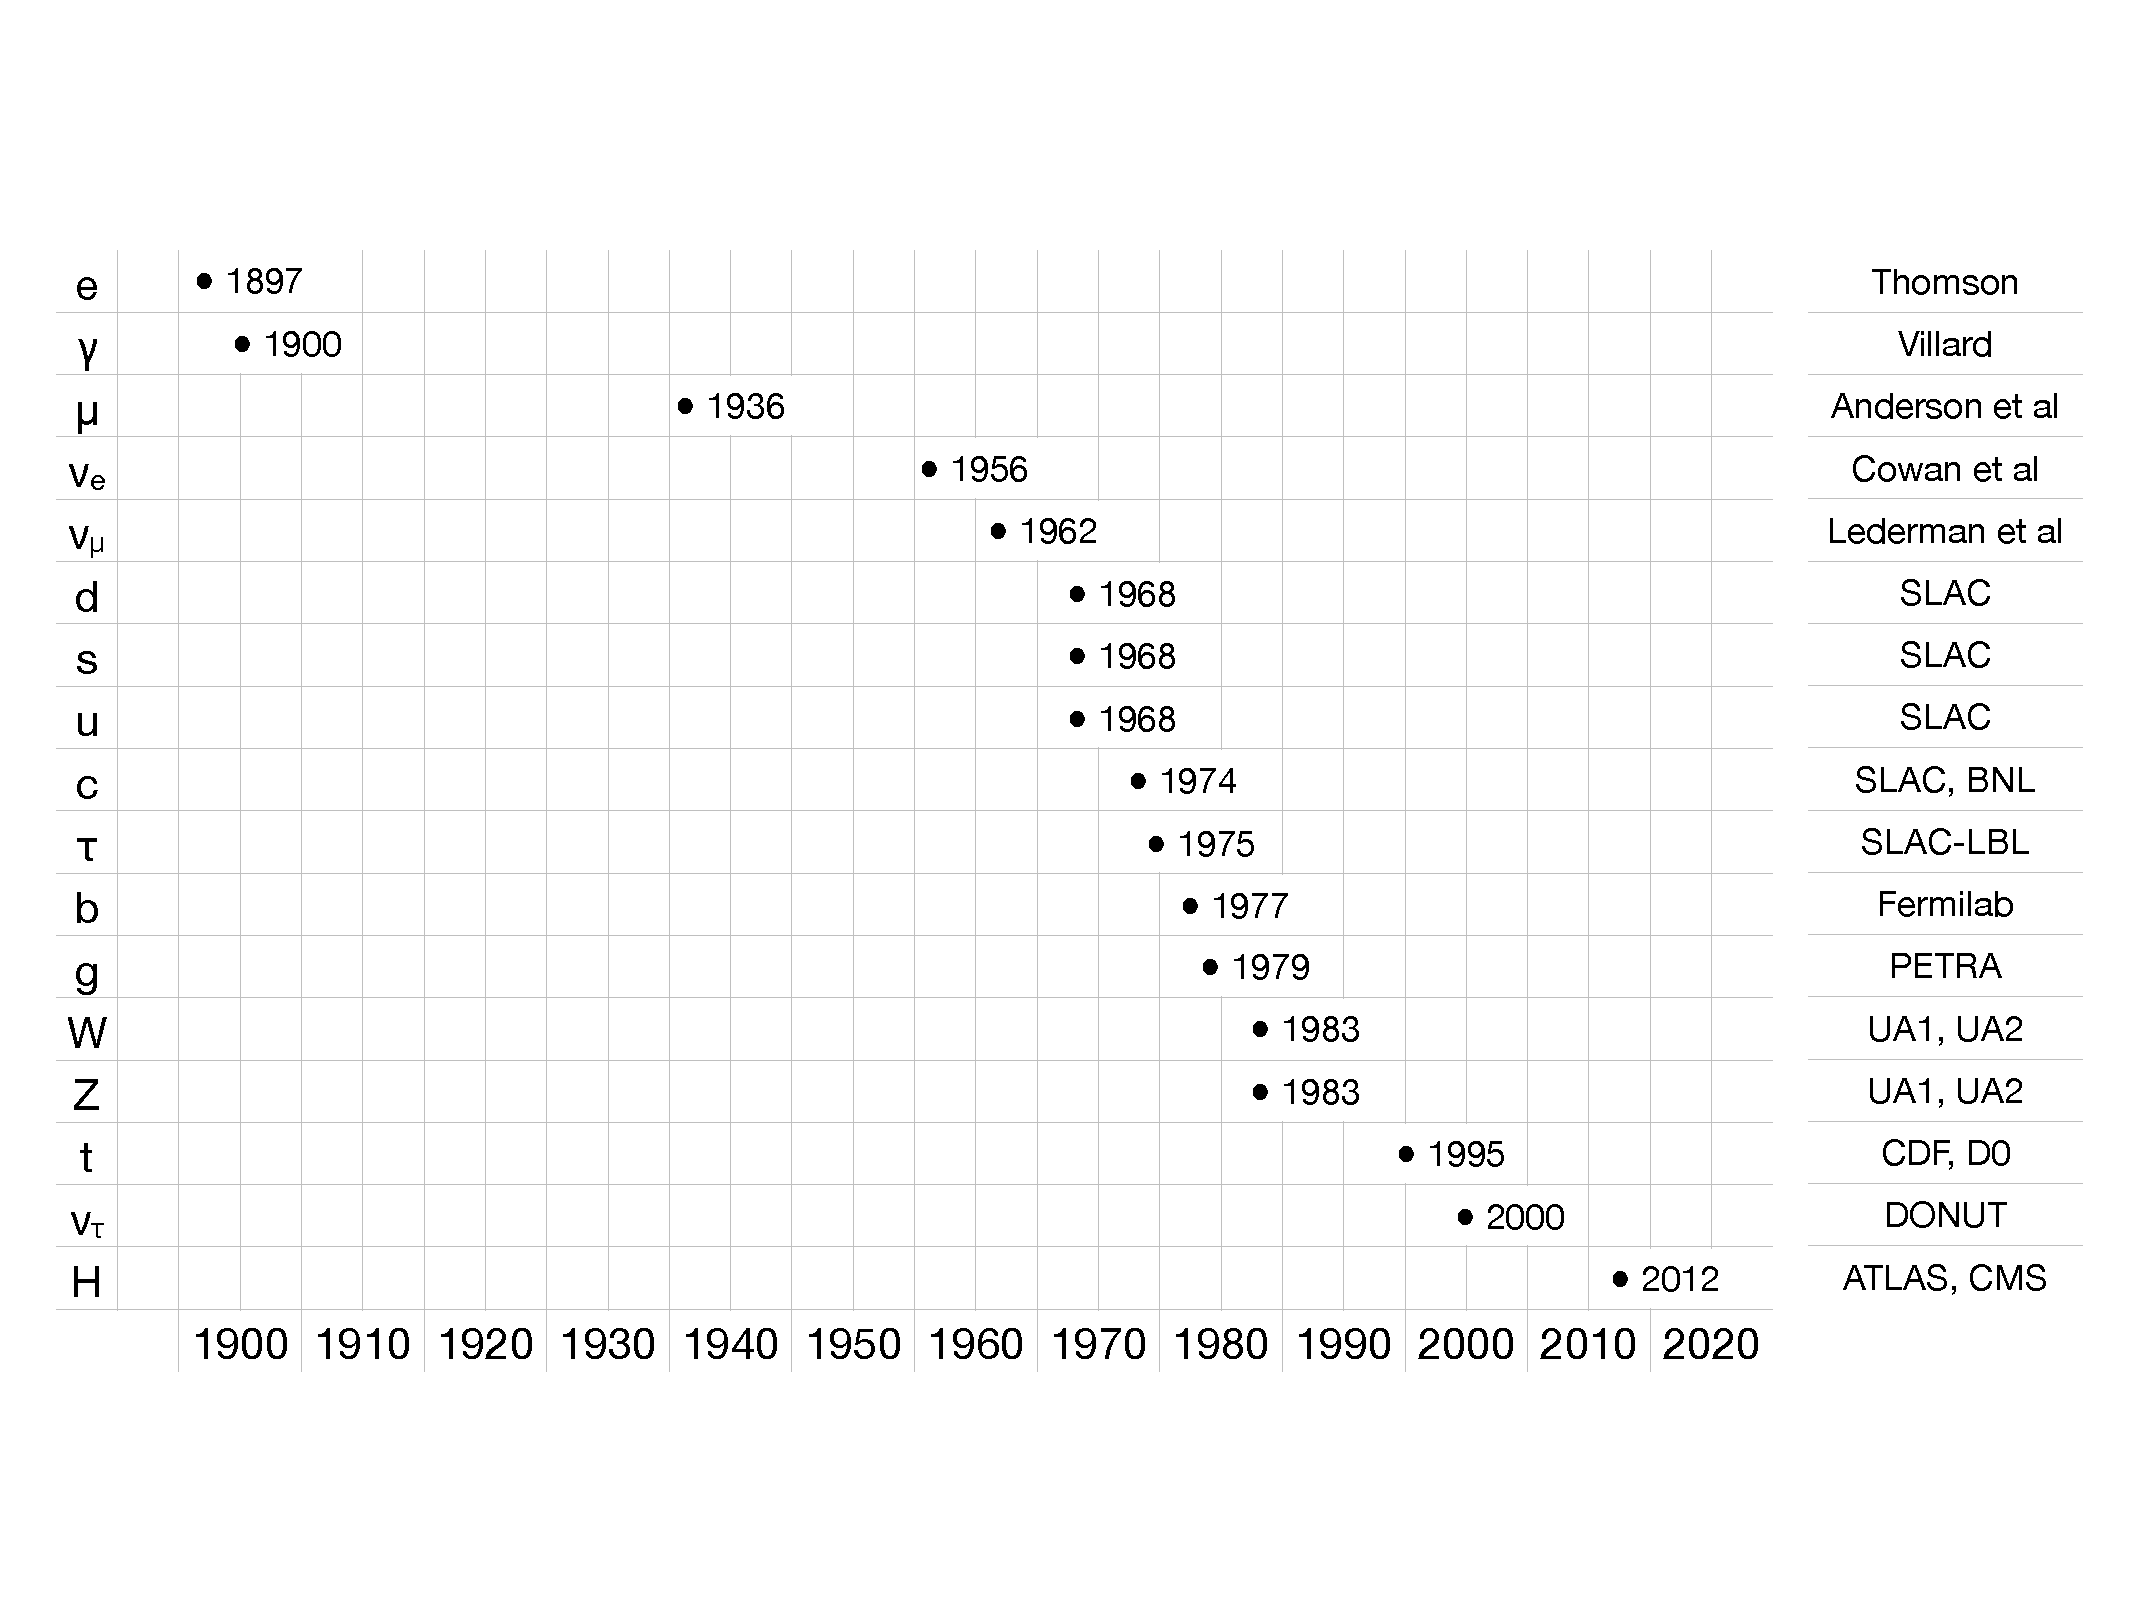
\includegraphics[width=0.90\textwidth]{figures/intro/discoveries.pdf}
      \end{center}
\caption{The discoveries of fundamental particles versus time~\cite{Tuna:thesis}.}
\label{fig:discoveries}
\end{figure}

In this theory, particles are treated as excitations of fields having half-integer spin or
integer spin, and the forces are treated as interactions among excitations of these fields.
The spin-$\frac{1}{2}$ particles, or fermions, can be divided into groups based on the ways
in which they interact. The leptons, or those particles which only experience the electroweak force,
are the electron $e$, muon $\mu$, tau $\tau$, electron neutrino $\nu_e$, muon neutrino $\nu_\mu$, and
tau neutrino $\nu_\tau$. The quarks, or those particles which experience both electroweak and strong
forces, are the up $u$, down $d$, strange $s$, charm $c$, bottom $b$, and top $t$. The integer-spin
particles, or bosons, are the spin-1 photon $\gamma$, $W$, $Z$, and gluon $g$ and the spin-0 Higgs $H$.
The particle content of the SM is summarized in Figure~\ref{fig:SMtable}.

\begin{figure}[ht]
 \begin{center}
    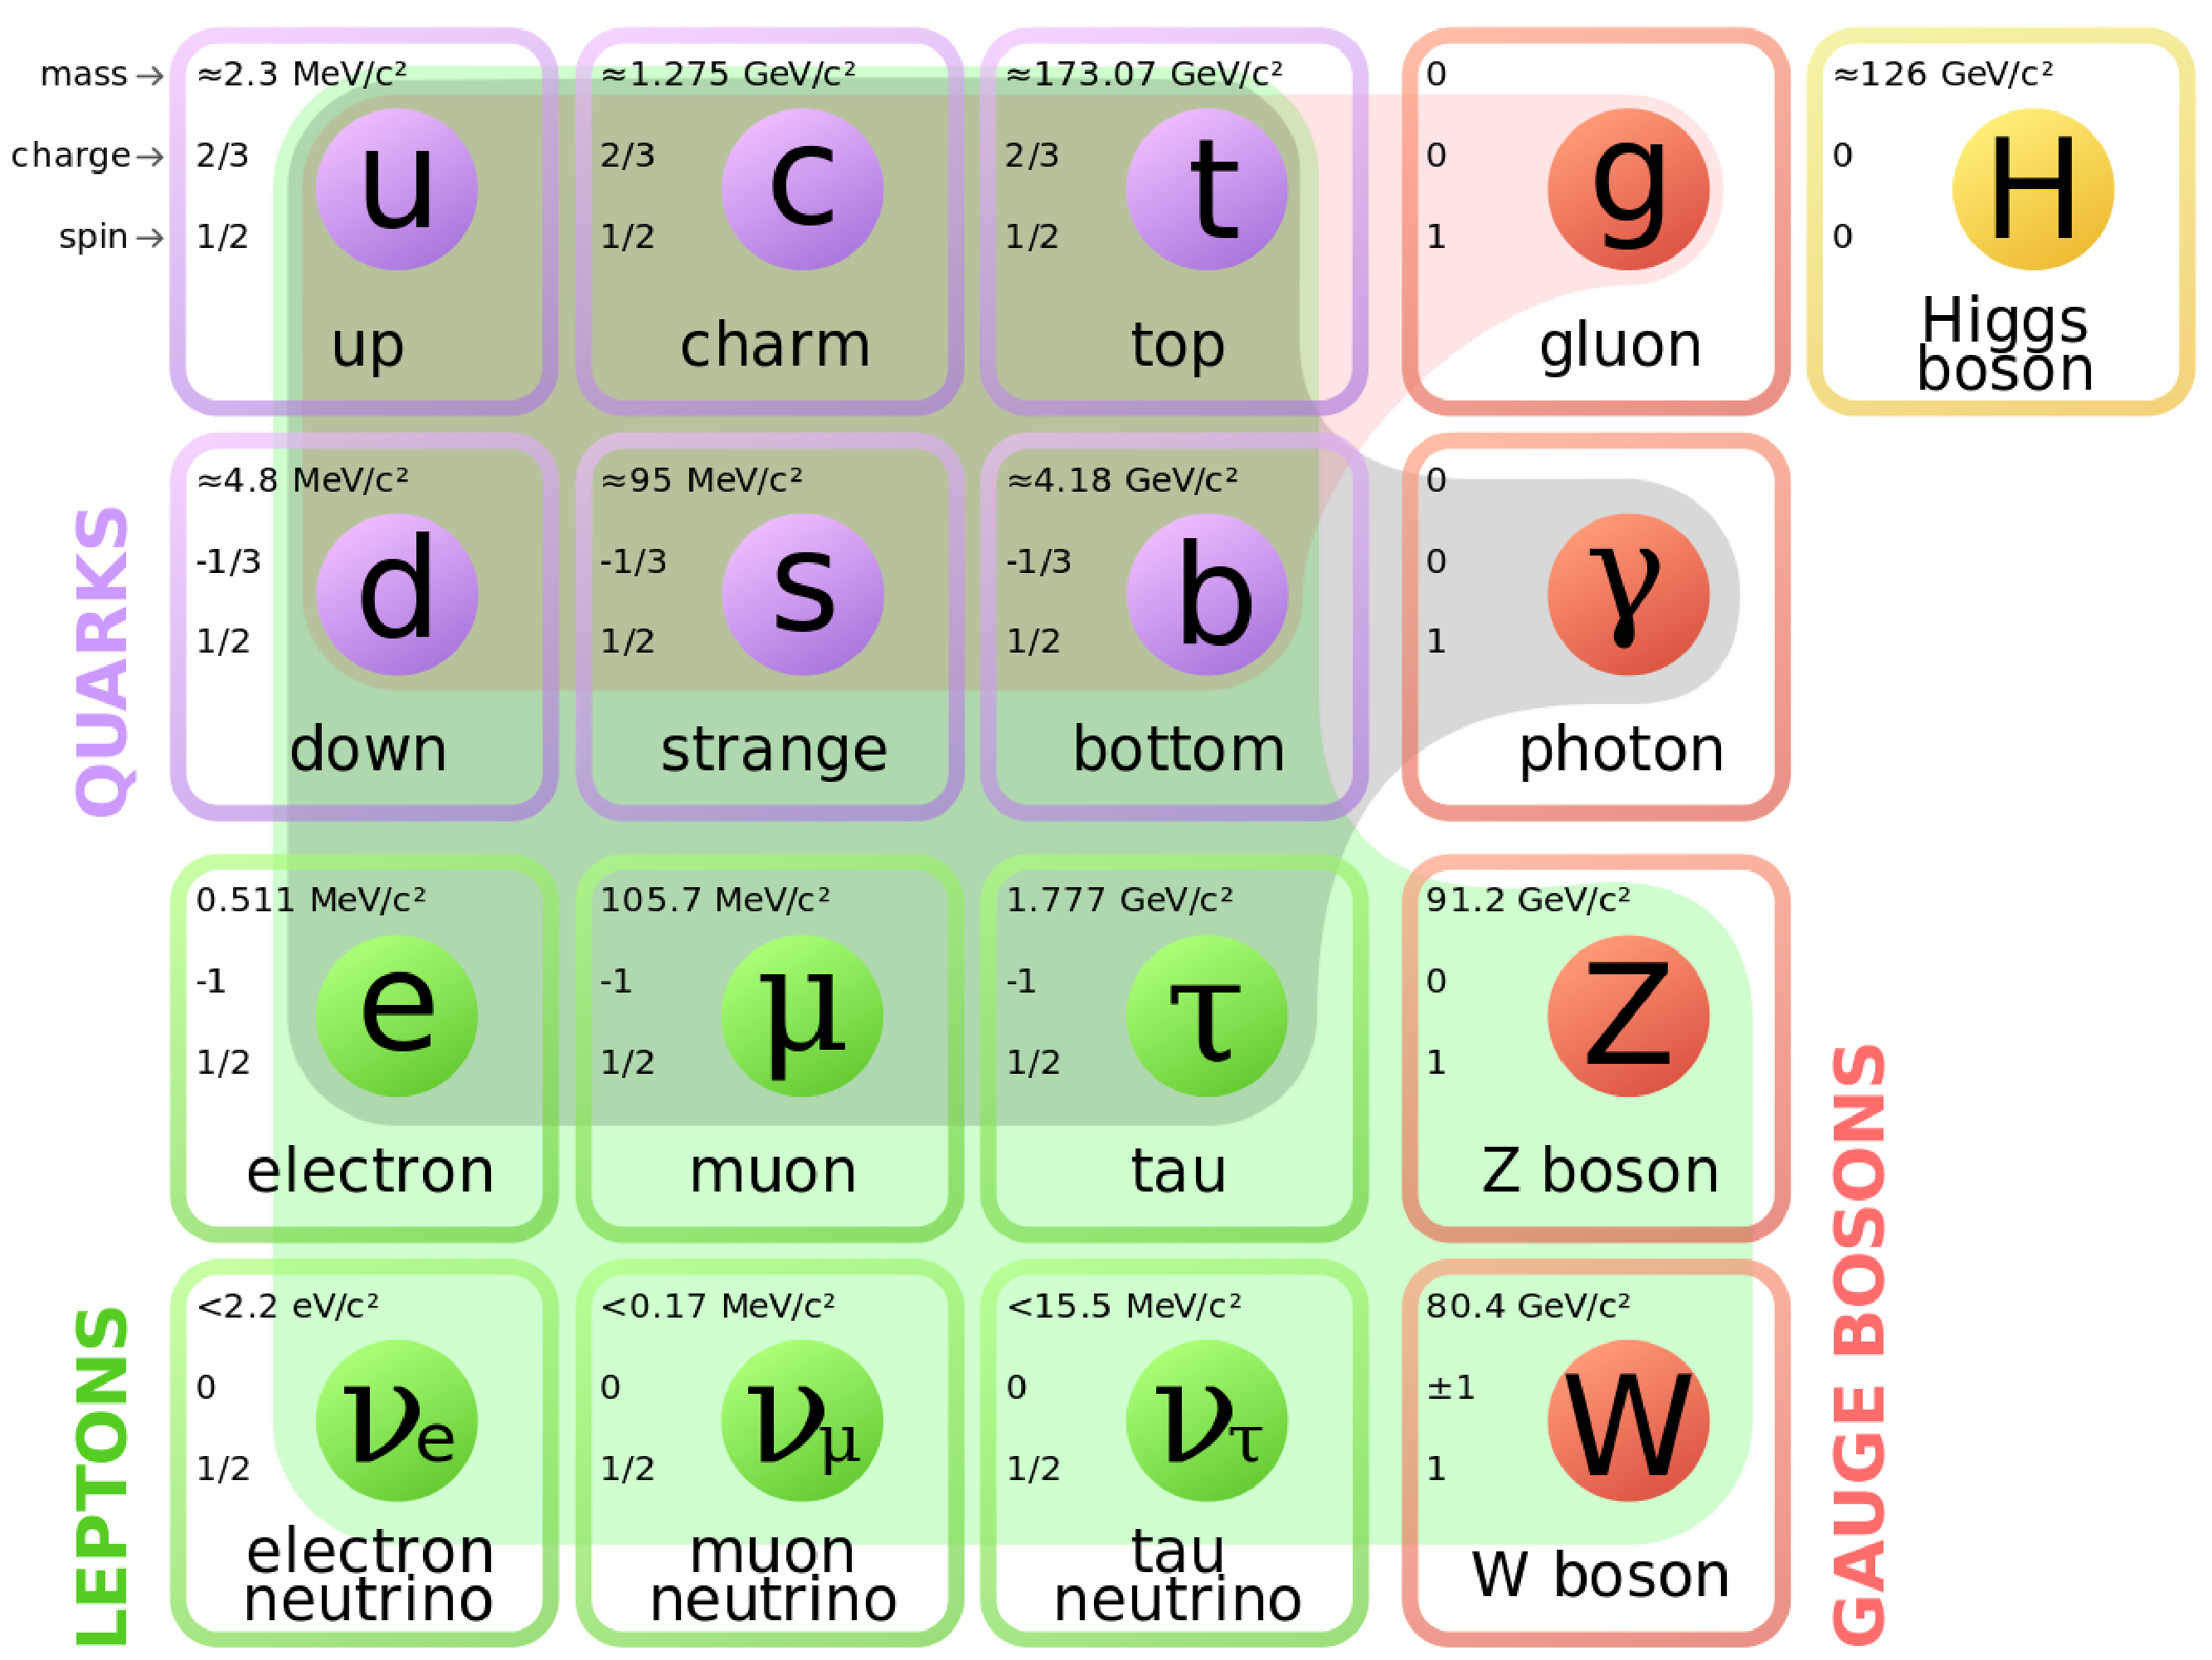
\includegraphics[width=0.80\textwidth]{figures/intro/Standard_Model_of_Elementary_Particles_modified_version.pdf}
      \end{center}
\caption{A diagram of the particle content of the SM~\cite{SMdiagram}.
The mass, electric charge, and spin is given for each, and the background color indicates how each
fermion interacts with the bosons.}
\label{fig:SMtable}
\end{figure}

The dynamics of the SM are described through its Lagrangian, which is invariant under
gauge transformations of the group ${\rm SU(3)}_C \times {\rm SU(2)}_L \times {\rm U(1)}_Y$.
The strong force, also known as quantum chronodynamics (QCD),
is associated with transformations under ${\rm SU(3)}_C$, which give rise to
the conserved color charge $C$, denoted red, green, or blue, and eight gauge fields.
The group acts on 18 spinor fields corresponding to the quarks (six quark flavors in three colors)
and the eight gauge fields corresponding to the gluons.
The electroweak force is associated with transformations under ${\rm SU(2)}_L \times {\rm U(1)}_Y$,
the first part of which give rise to the conserved left-handed chirality $L$ and three gauge fields,
and the second part of which gives rise to the conserved weak hypercharge $Y$ one gauge field.
This group acts on left-handed doublets and right-handed singlets of the quarks, leptons, and
these four gauge fields. The quarks contribute nine doublets and 18 singlets, and the leptons contribute
three doublets and three singlets (as right-handed neutrinos do not exist).

The symmetry group of the SM does not allow for gauge-invariant mass terms. Instead,
the generation of particle masses is accomplished through the partial breaking of the
symmetry group by the addition of the Higgs field and potential, after which gauge-invariant
Yukawa interactions between fermions and the Higgs field naturally give fermion masses.
The Higgs field $\phi$ is a doublet of ${\rm SU(2)}_L$, and its potential takes the form
\begin{equation}
V(\phi^\dagger\phi) = -\mu\phi^\dagger\phi + \lambda(\phi^\dagger\phi)^2 \,,
\end{equation}
where $\mu,\lambda > 0$. The ground state of this potential is nonzero and degenerate. With the
choice of a convenient gauge, the ground state can be expressed as
\begin{equation}
\left\langle \phi \right\rangle =
\left\langle \frac{1}{\sqrt{2}} {\phi^0+i\phi^1 \choose \phi^2+i\phi^3} \right\rangle =
{\mu / \sqrt{\lambda} \choose 0} \,,
\end{equation}
where $\phi^1, \phi^2, \phi^3$ are massless Goldstone
bosons~\cite{1961.Goldstone,1962.Goldstone-Salam-Weinberg.Broken-Symmetries} and the remaining
degree of freedom represents fluctuations about this ground state,
associated with the massive scalar Higgs boson $H$.

Recalling that the Higgs field is a doublet of ${\rm SU(2)}_L$, its covariant derivative in the
Langrangian is
\begin{equation}
D_\mu = \partial_\mu - i g_1 T^a W^a_\mu - i \frac{g_2}{2} B_\mu \,,
\end{equation}
where $g_1$ ($g_2$) and $W^a_\mu$ ($B_\mu$) are the gauge couplings and three (one) gauge bosons
associated with ${\rm SU(2)}_L$ (${\rm U(1)}_Y$), respectively, and $T^a$ are the generators of
${\rm SU(2)}_L$. The ground state of the Higgs field then gives mass terms to some of the gauge bosons.
The mass eigenstates, in terms of the $W^a_\mu$ and $B_\mu$, are the $W^\pm$, $Z$, and photon with
masses
\begin{subequations}
\begin{equation}
m_{W^\pm} = \frac{g_1}{2}\frac{\mu}{\sqrt{\lambda}}
\end{equation}
\begin{equation}
m_Z = \frac{\sqrt{g_1^2+g_2^2}}{2}\frac{\mu}{\sqrt{\lambda}}
\end{equation}
\begin{equation}
m_\gamma = 0 \,.
\end{equation}
\end{subequations}
Thus, the gauge bosons acquire mass, and the symmetry of ${\rm SU(2)}_L \times {\rm U(1)}_Y$ is
broken to ${\rm U(1)}_{EM}$ with gauge field being the photon.  

Masses for the fermions are generated through this symmetry breaking through the introduction of
gauge-invariant interactions with the Higgs field into the Lagrangian. These take the form
\begin{equation}
\mathcal{L}_{\text{Yukawa}} = -g \bar{\psi}\phi\psi \,,
\end{equation}
where $g$ is the strength of the interaction. Here, the symmetry breaking caused by
$\phi \rightarrow \left\langle \phi \right\rangle + H$ gives a mass term of the form
$g \left\langle \phi \right\rangle$ and an interaction with the Higgs boson. Interactions with the
other bosons arise from change in the covariant derivative of each fermion field due to the
symmetry breaking.

These interactions can be represented pictorially with
Feynman diagrams~\cite{1948.Feynman.path-integral-QM}. Figure~\ref{fig:nonhiggsint} shows the
interaction vertices of the SM in which the Higgs is not involved. These diagrams provide a powerful
tool for the calculation of probability amplitudes of SM processes, which are directly related to the
experimentally-measurable cross sections.

\begin{figure}[ht]
 \begin{center}
    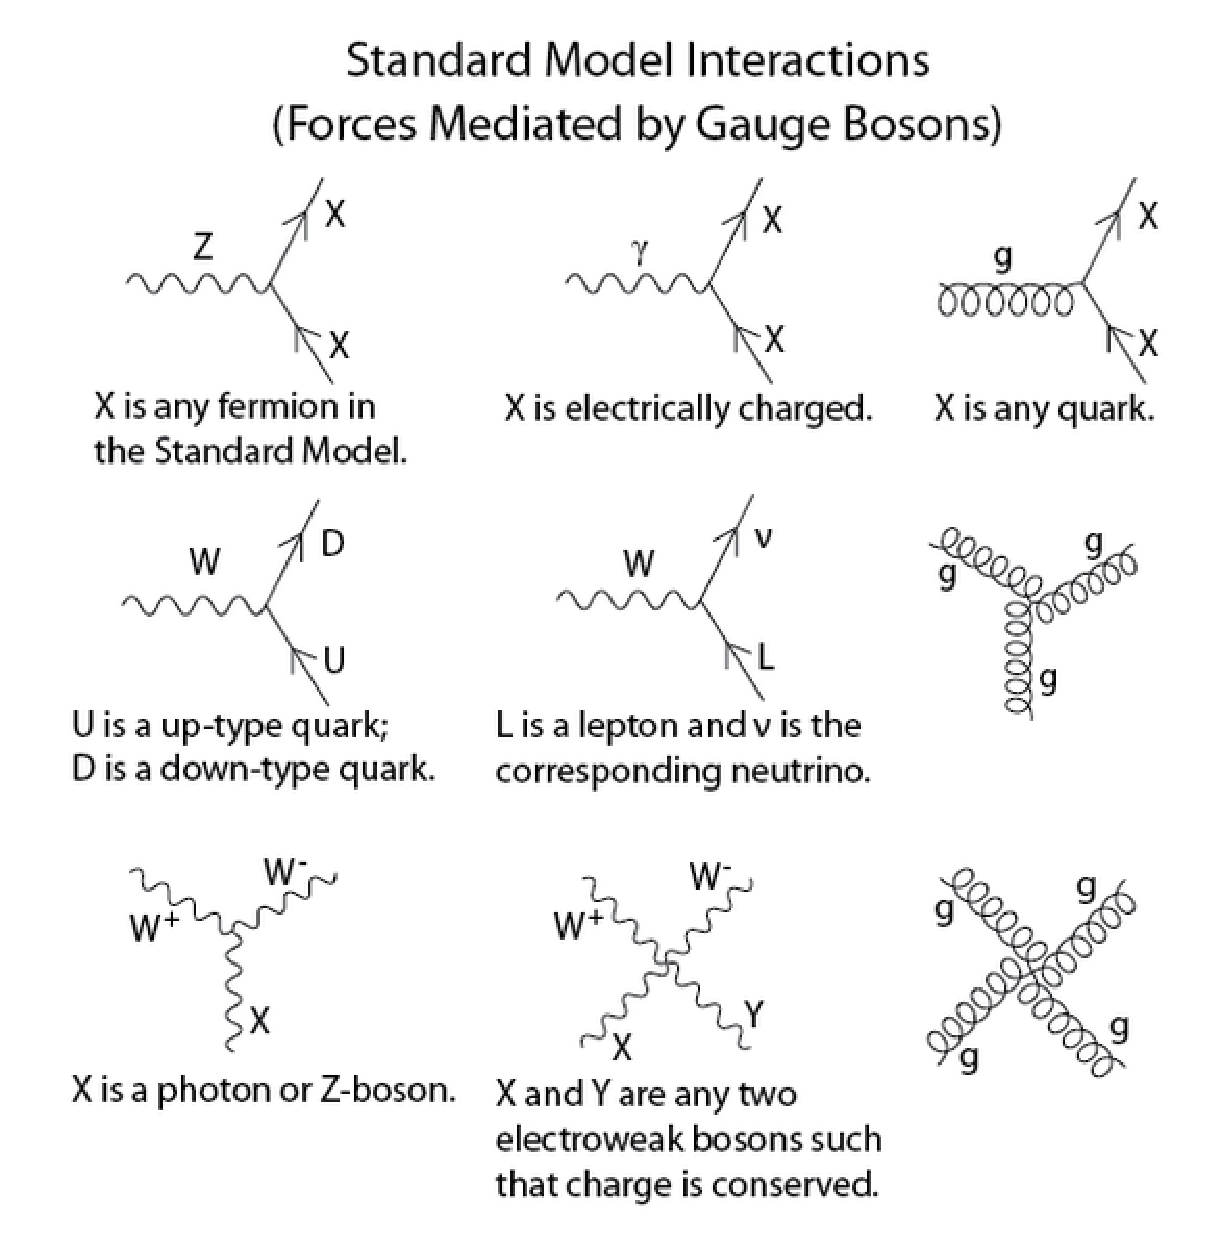
\includegraphics[width=0.80\textwidth]{figures/intro/Standard_Model_Feynman_Diagram_Vertices.pdf}
      \end{center}
\caption{Interactions of the SM in which the Higgs in not involved~\cite{SMinteractions_nonhiggs}.}
\label{fig:nonhiggsint}
\end{figure}

\section{Higgs Discovery\label{sec:discovery}}

While each particle has its own story of discovery, as hinted briefly by Figure~\ref{fig:discoveries},
this section will focus on the technical details related to that of the Higgs.
What makes the search especially difficult is the
small couplings that the Higgs has with other particles, as shown in Figure~\ref{fig:crosssections}.
However, up until 2012, the mass of the Higgs boson was unknown, so big experimental searches
had to accommodate a wide range of possible values.

\begin{figure}[ht]
 \begin{center}
    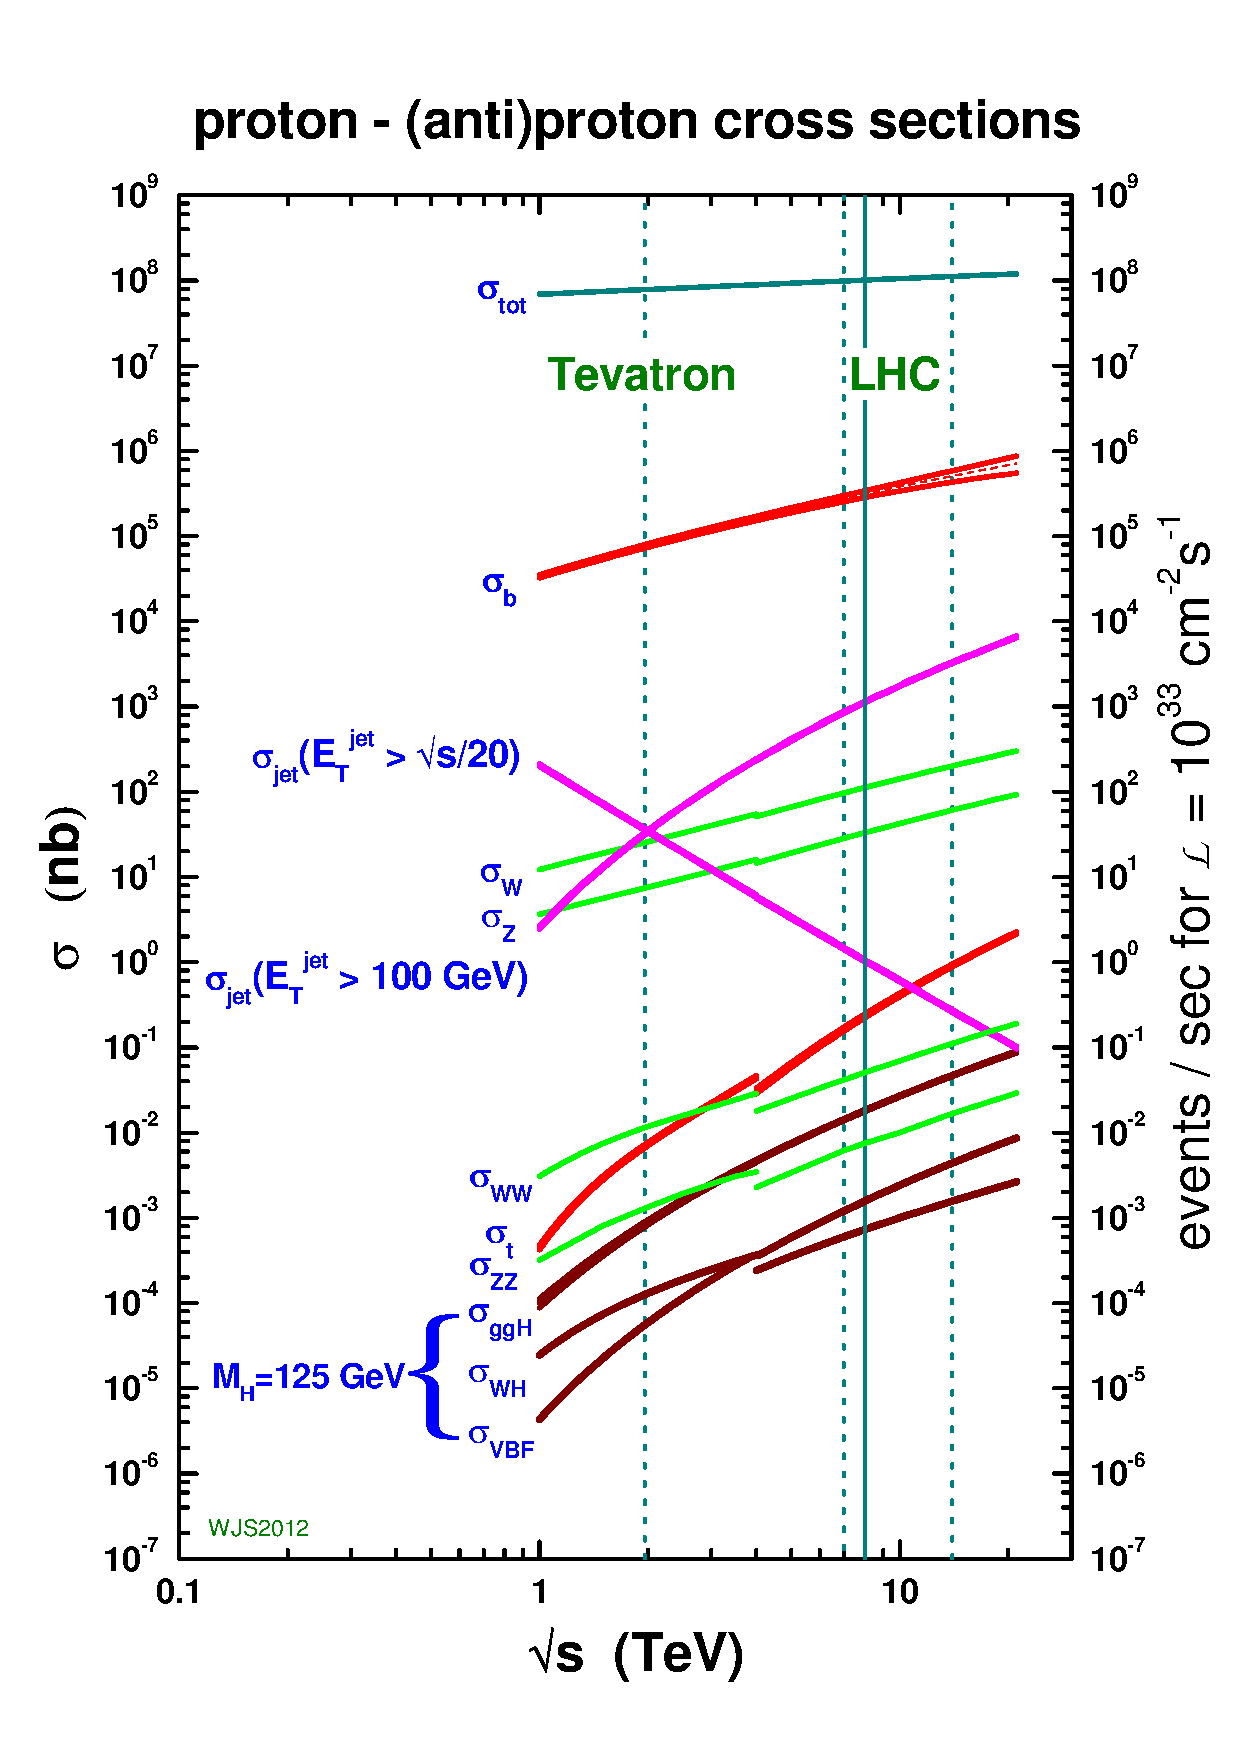
\includegraphics[width=0.70\textwidth]{figures/intro/crosssections2012_v5.pdf}
      \end{center}
\caption{Production cross sections for various processes in the SM versus center-of-mass energy.
The lower energies correspond to $p\bar{p}$ collisions from the Tevatron~\cite{Group:1984bk}, whereas
the higher energies correspond to $pp$ collisions from the LHC~\cite{cern-jinst-lhc}.}
\label{fig:crosssections}
\end{figure}

The search for the Higgs can be broken down into production mechanism and decay mode. For $pp$
collisions at $\sqrt{s} = 8$~TeV, as realized at the LHC (see Section~\ref{sec:LHC}),
Figure~\ref{fig:higgsprod} shows the
dominant production mechanisms and corresponding cross sections. The branching ratios for several
of the dominant decay modes are given in Table~\ref{table:BR_SMhiggs}.

\begin{figure}[ht]
 \begin{center}
    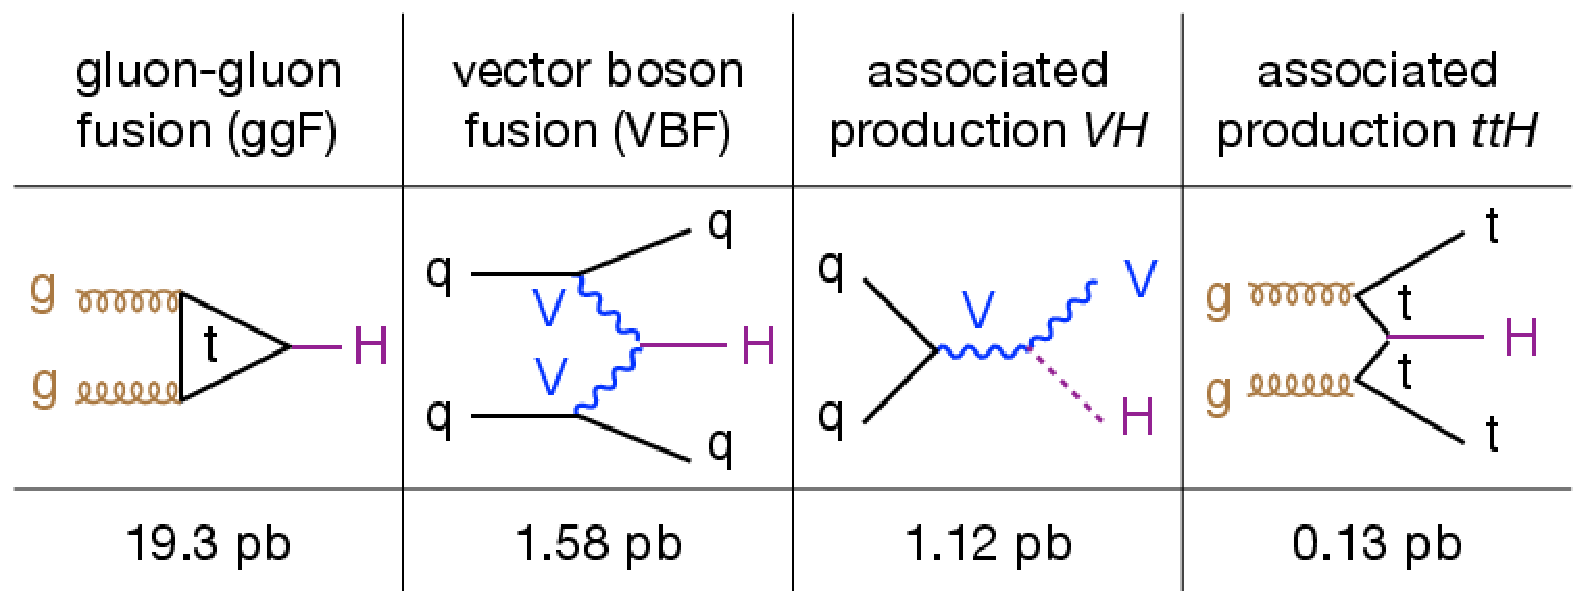
\includegraphics[width=0.90\textwidth]{figures/intro/higgsproductions.pdf}
      \end{center}
\caption{Production mechanisms and cross sections of the Higgs boson
for the leading processes in the SM~\cite{Tuna:thesis}. The cross sections correspond to
$pp$ collisions at $\sqrt{s} = 8$~TeV.}
\label{fig:higgsprod}
\end{figure}

Since the announcement of discovery of a new Higgs-like particle
in 2012~\cite{higgsdiscoveryAtlas,Chatrchyan:2012ufa}, the properties of the Higgs have been narrowed
through the accumulation of more data and more refined analyses~\cite{Hdiscovery}. The general
conclusion of all these analyses is that the Higgs boson is, up to the sensitivity that the present
dataset allows, consistent with that predicted by the SM. Figures~\ref{fig:measuredxsec_prod} and
\ref{fig:measuredxsec_decay} provide two of these highlights in $\mu$ for each of the
production cross sections and decay modes, respectively, where $\mu$ is the
ratio of the measured cross section to that predicted by the SM.

\begin{table}[ht]
  \centering
  \renewcommand{\arraystretch}{1.4}
  \caption{Branching ratios for the Higgs boson~\cite{LHC:SMHiggsBR}.}
  \begin{tabular}{|c|ccc|cccc|}
\hline
                     & \multicolumn{3}{c|}{fermions} & \multicolumn{4}{c}{bosons}  \\
  \hline
  Decay mode         & $bb$ & $\tau\tau$ & $\mu\mu$   & $WW^\ast$ & $ZZ^\ast$ & $\gamma\gamma$ & $Z\gamma$ \\
  Branching fraction & 58\% & 6.3\%     & 0.022\%    & 22\%      & 2.6\%     & 0.23\%         & 0.15\%    \\
\hline
\end{tabular}

  \label{table:BR_SMhiggs}
\end{table}

\begin{figure}[ht]
 \begin{center}
    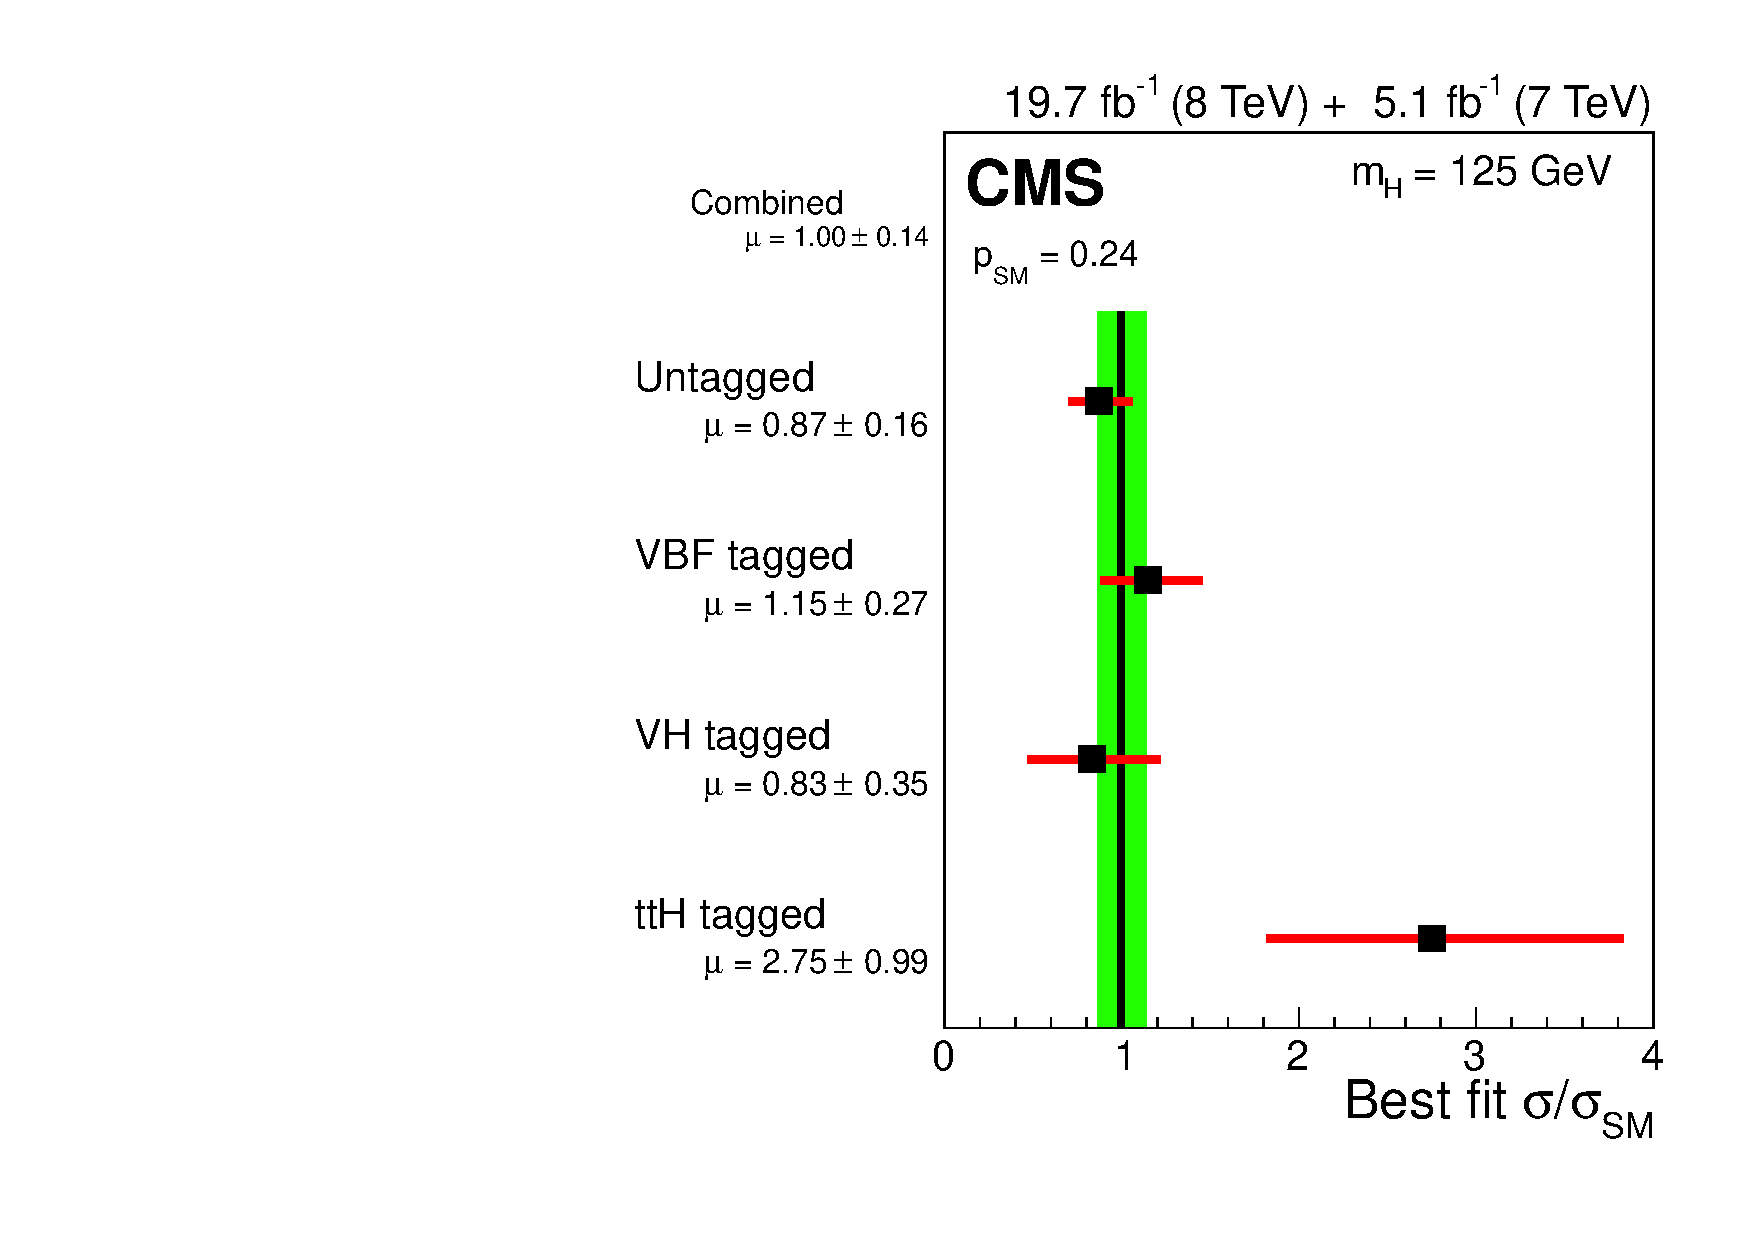
\includegraphics[width=0.55\textwidth]{figures/intro/sqr_mlz_ccc_mH125_prod.pdf}
      \end{center}
\caption{Values of the best-fit $\mu$ for the combination (solid vertical line) and for
subcombinations by analysis tags targeting individual production mechanisms~\cite{Khachatryan:1979247}.
The vertical band shows the overall $\mu$ uncertainty. The $\mu$ ratio denotes the production cross section times the relevant branching ratios, relative to the SM expectation. The horizontal bars indicate the $\pm 1$ standard deviation uncertainties in the best-fit $\mu$ values for the individual modes; they include both statistical and systematic uncertainties.}
\label{fig:measuredxsec_prod}
\end{figure}

\begin{figure}[ht]
 \begin{center}
    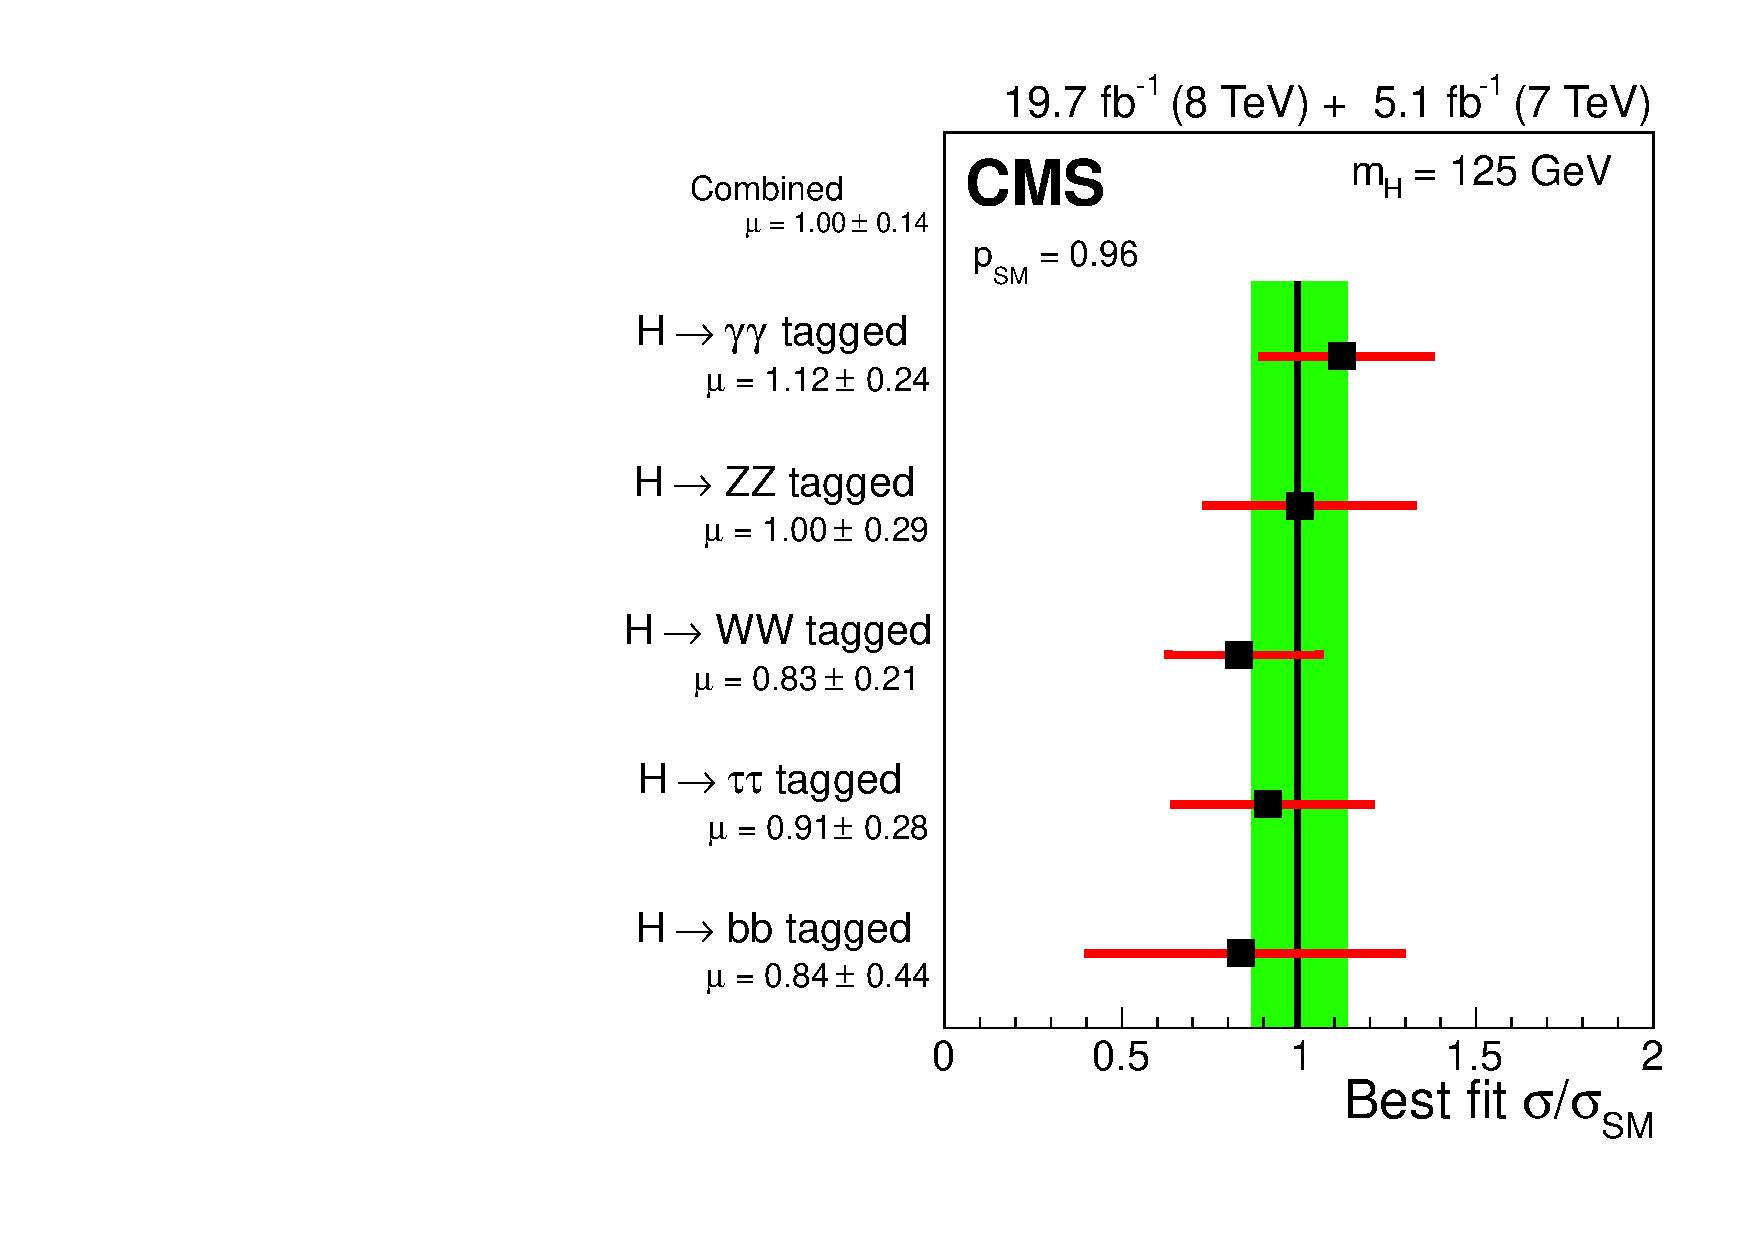
\includegraphics[width=0.55\textwidth]{figures/intro/sqr_mlz_ccc_mH125_decay.pdf}
      \end{center}
\caption{Values of the best-fit $\mu$ for the combination (solid vertical line) and for subcombinations by predominant decay mode~\cite{Khachatryan:1979247}. The vertical band shows the overall $\mu$ uncertainty. The $\mu$ ratio denotes the production cross section times the relevant branching ratios, relative to the SM expectation. The horizontal bars indicate the ±1 standard deviation uncertainties in the best-fit $\mu$ values for the individual modes; they include both statistical and systematic uncertainties.}
\label{fig:measuredxsec_decay}
\end{figure}

Perhaps the most important measurement from the discovery is that of the Higgs boson mass.
Figure~\ref{fig:measuredmass} provides experimental evidence for the precision measurement of this
value by considering only high-resolution channels for Higgs boson production and decay.
The measured value is around 125 GeV. This provides a means to probe other features of the SM
or to search for signatures of physics beyond the SM (BSM). One of those processes, which
is the major topic of interest for this thesis, are searches in which two Higgs bosons are produced.
The theoretical grounds for such processes are discussed in
Section~\ref{sec:diHiggs}.


\begin{figure}[ht]
 \begin{center}
    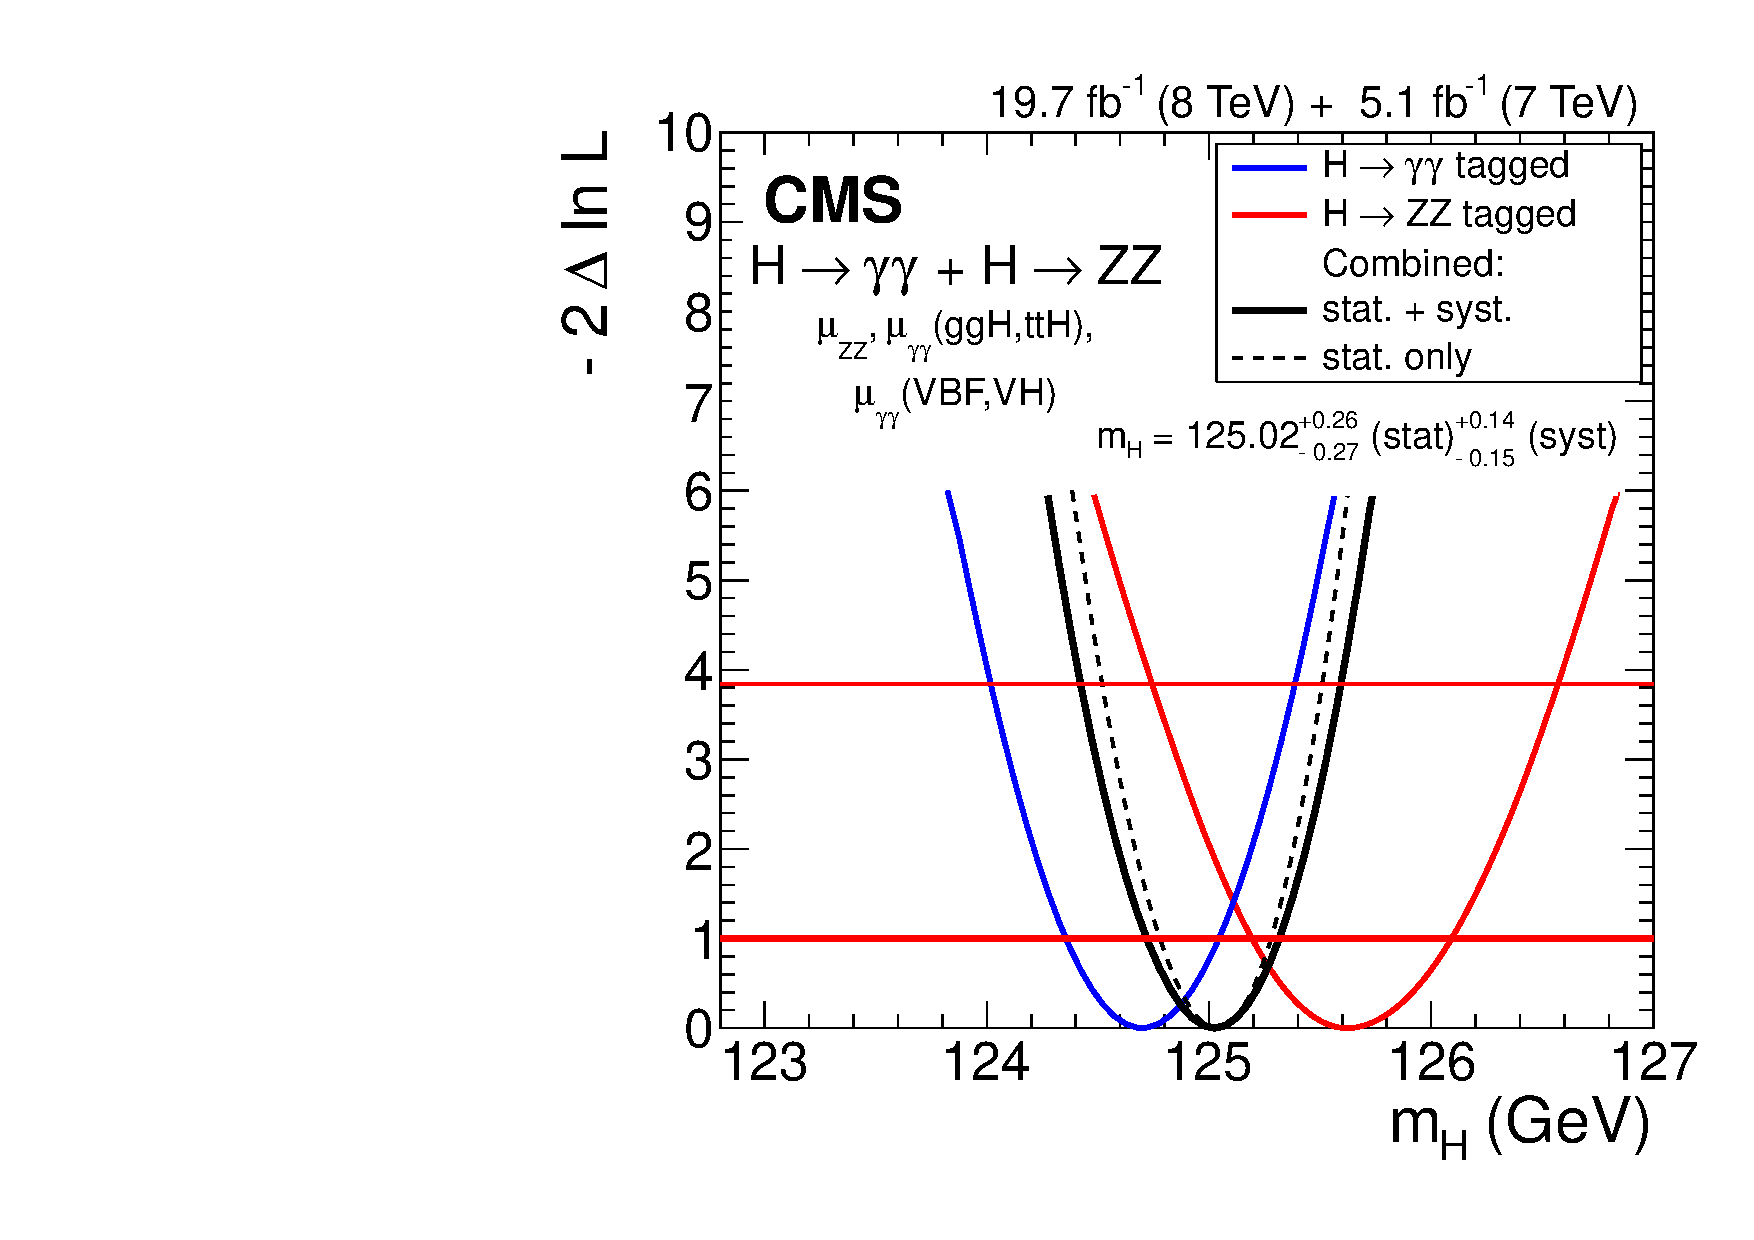
\includegraphics[width=0.55\textwidth]{figures/intro/sqr_mass_all.pdf}
      \end{center}
\caption{Scan of the test statistic $q(m_H)=−2\Delta\log{L}$ versus the mass of the boson $m_H$ for the $H\rightarrow\gamma\gamma$ and $H\rightarrow ZZ\rightarrow 4\ell$ final states separately and for their combination~\cite{Khachatryan:1979247}. Three independent signal strengths, (ggH,ttH)$\rightarrow\gamma\gamma$, (VBF,VH)$\rightarrow\gamma\gamma$, and $pp\rightarrow H\rightarrow ZZ\rightarrow 4\ell$, are profiled together with all other nuisance parameters. The solid curve is obtained by profiling all nuisance parameters and thus includes both statistical and systematic uncertainties. The dashed curve is obtained by fixing all nuisance parameters to their best-fit values, except for those related to the $H\rightarrow\gamma\gamma$ background description, thus including only statistical uncertainties. The crossings with the thick (thin) horizontal lines define the 68\% (95\%) CL interval for the measured mass. }
\label{fig:measuredmass}
\end{figure}



\section{Shortcomings of the SM\label{sec:SMshortcomings}}

There are both experimental and theoretical reasons for why the SM is not a complete theory of
particle physics. In some cases, the SM provides an ad-hoc description, and in other cases, there
is no description at all. For the optimist, these provide compelling reasons to continue
pushing the boundaries of our knowledge. Examples of such compelling questions concern gravity,
dark matter, dark energy, and neutrinos, as detailed in Subsections~\ref{subsec:grav},
\ref{subsec:dark}, and \ref{subsec:neu}, but this is not to omit other questions concerning,
for example, matter-antimatter asymmetry, hierarchy, naturalness,
dark energy, and the generations of fermions.

\subsection{Gravity\label{subsec:grav}}

Gravity is well understood in the classical and relativistic limits, as first posited by Newton
and Einstein, respectively. However, there is no complete quantum theory of gravity, and as such
it is not accounted for by the SM. It is thought that the force is mediated by a spin-2 particle
called the graviton and that the gravitational force would unify with the other three forces
in a very-high energy limit.

\subsection{Dark Matter\label{subsec:dark}}

Ordinary matter, as built-up from the SM, only accounts for 15\% of the
matter in the universe~\cite{Clowe:2006eq}. The nature of the other 85\%, dubbed dark matter, is
largely unknown. Its presence is inferred from observing the way ordinary matter behaves at
astrophysical scales. In these observations, the behavior of certain objects cannot be explained
by the ordinary matter alone. Rather, it is posited that these observations can be explained by
the presence of some additional matter which interacts through gravity but not electromagnetism.
Candidate dark matter particles provide motivation for many experimental searches at the LHC and
other experiments.

\subsection{Neutrinos\label{subsec:neu}}

In the version of the SM presented in~\ref{sec:SM}, neutrinos are massless, electrically neutral
leptons which come in three flavors. The observation of neutrino oscillation~\cite{Fukuda:1998mi},
in which the probability of measuring a particular flavor in a neutrino varies over its trajectory,
implies that neutrinos have masses. These mass terms can and have been added to the SM, but it is
unclear if their origin is from the same mechanism that provides the other fermions with their
masses.

\section{Double Higgs as a probe of SM and New Physics\label{sec:diHiggs}}

With the mass of the Higgs known, searches involving the production of two Higgs bosons may
be performed. The principle motivation for searching for such a process is two-fold.
It provides a means for searching for an interaction predicted by the SM but not yet observed, that
of the Higgs trilinear coupling, which provides further understanding of the Higgs potential.
While searching for this rare SM process, similar topologies involving BSM physics may
be sought. The goal of the latter would be to either find a deviation from what the SM predicts
or to place limits on the extent to which new theories may be excluded.

Double Higgs production at hadron colliders in the SM has been studied
theoretically~\cite{Baglio:2012np,Plehn:1996wb}, and the cross section for $pp$ collisions at 8 TeV
is 9.96 fb level (including NNLO corrections). This is unfortunately out of reach of current
experiments, and it is due, in part, to the destructive interference exhibited between contributions
from the the Higgs self-coupling and from a top-loop with two Higgs, as shown in
Figure~\ref{fig:diHiggs_diagrams}.

If the couplings from the diagrams in Figure~\ref{fig:diHiggs_diagrams} were to not take their SM
values, an the double Higgs cross section could be enhanced, leading to possible sensitivity
at current experiments. These kinds of effects are present in models
where the Higgs is interpreted as a composite state of some strong dynamics. The deviations
of the SM couplings that could arise from the simpler composite Higgs case are
already very constrained~\cite{Ellis:2013ywa,Ellis:2013lra}.
However, under more general assumptions, higher order
operators could in principle lead to sizable effects~\cite{Belyaev:1999mx,Dib:2005re,Oliveira:2010uv}.
This possibility is discussed in Subsection~\ref{subsec:nonres_th}.

\begin{figure}
\begin{center}
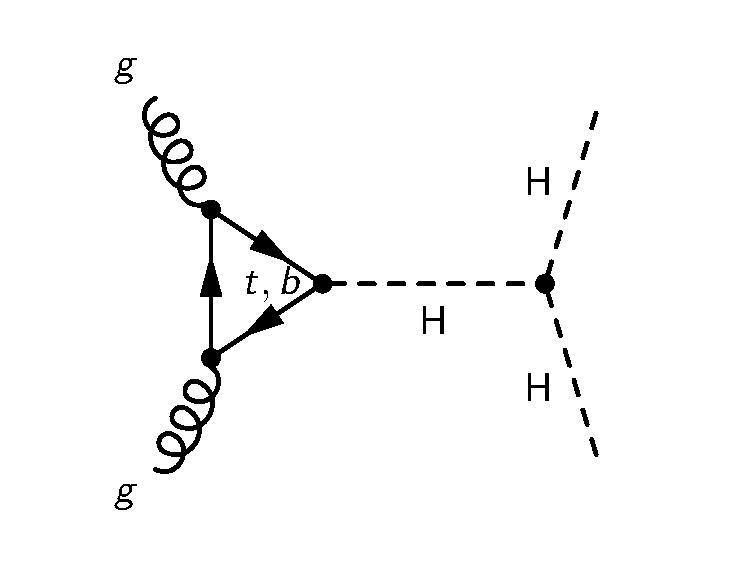
\includegraphics[width=.32\textwidth]{figures/intro/diHiggs_lambda.pdf}
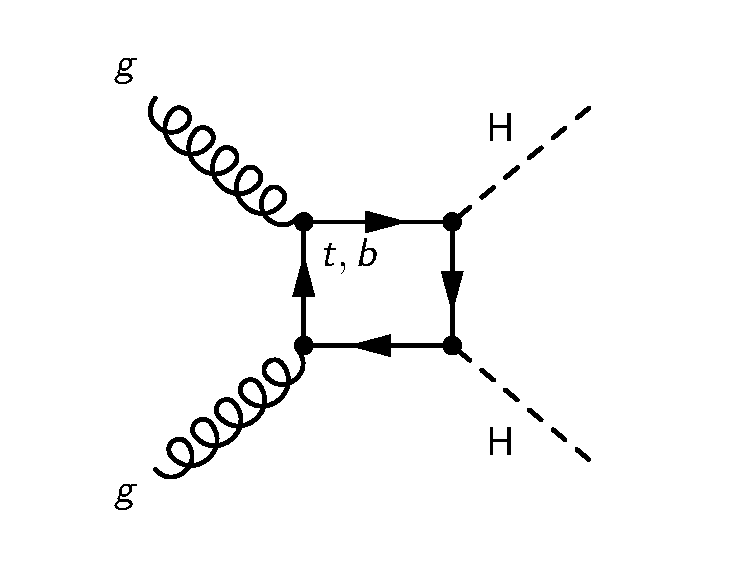
\includegraphics[width=.32\textwidth]{figures/intro/diHiggs_yt.pdf}
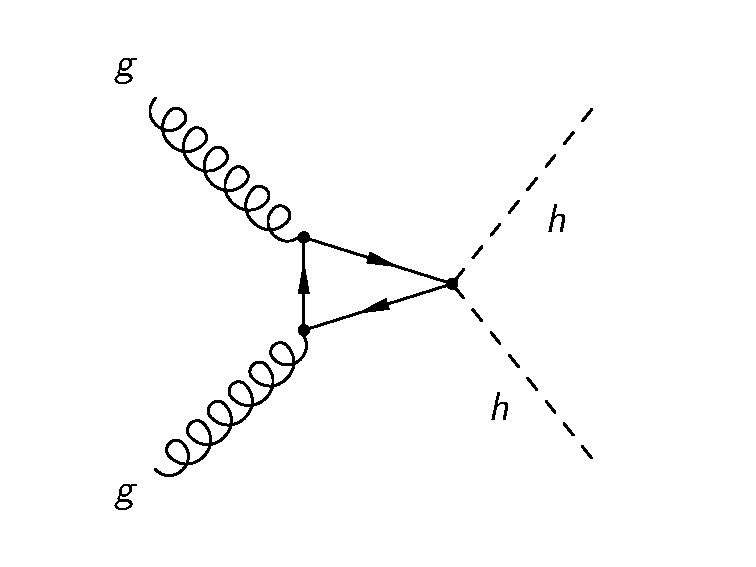
\includegraphics[width=.32\textwidth]{figures/intro/diHiggs_c2.pdf}
\end{center}
\caption{
\label{fig:diHiggs_diagrams}
Feynman diagrams of the processes responsible for non-resonant gluon fusion production of two
Higgs bosons in the final state.
These diagrams involve the Higgs boson self-coupling (left), the top quark Yukawa coupling (middle),
predicted in the case of the Standard Model,
as well as the anomalous coupling $ttHH$ (right) which is open in case of an effective
parametrization of the Lagrangian by dimension 6 operators.}
\end{figure}

Double Higgs production can also be used to search for the presence of a new, heavy particle
with spin of 0 or 2 and with
mass at least double $m_H$ so that decay to $HH$ is kinematically allowed. Such new particles
can be motivated from BSM scenarios which typically have dominant decay modes to pairs of
$W$s, $Z$s, tops, and Higgs. Some of these scenarios are discussed briefly in
Subsection~\ref{subsec:res_th}.

\subsection{Nonresonant Double Higgs Production from BSM\label{subsec:nonres_th}}

In this thesis, nonresonant double Higgs production is parametrized by the Higgs trilinear
self-coupling $\lambda$, the Yukawa top coupling $y_t$, and an anomalous $t\bar{t}HH$ coupling $c_2$.
The potential of the Higgs and its interactions with the top quark can be written as

\begin{equation}
\begin{split}
\Delta L_{H,t;y_t,c_2}= 
\partial_{\mu}\, H \partial^{\mu} H - m_H H^2 +
\kappa_{\lambda}\, \lambda_{SM} v\, H^3 \\
- \frac{\sqrt{2} m_t}{v}(v+  \kapt\,   H  +  \frac{ \sqrt{2}\, c_2}{v} H  H ) \,( \bar{t_L}t_R + h.c.)  \,,
\end{split}
\label{eq:Hpot}
\end{equation}
where $v = 246 \mbox{ GeV}$, $\lambda_{SM} \equiv \frac{m_H^2}{2 v^2} = 0.129$, and
$y_{t,SM} = \frac{\sqrt{2} m_t}{v} = 0.995$. Possible contact interactions between the
Higgs and gluons that could arise from heavy coloured scalars are neglected.
Only dimension-6 operators are relevant to BSM physics. The parameters $c_2$ and $y_t$ are
analytically related by the coefficients of two dimension six operators, one being the
derivative of the interaction among four Higgs doublets with coefficient $c_H$
and the other involving the interactions between the Higgs doublet and top quarks
with coefficient $c_t$.

For the interpretation of the BSM nonresonant search, the LO cross section for double Higgs production
is expressed in a semi-analytical form~\cite{Contino:2012xk}
%, In this reference the coeficients in Equation \ref{eq:coefnonres} are calculated by numerical integration of the matrix element developed by the authors. In our work however we prefer to re-
%The result of our parameters fit is found in Equation \ref{eq:coefnonres}.
\begin{equation}
\begin{split}
\sigma (pp\to HH) = \bar{\sigma} [  \ctwo^2 + (\alpha \kapt^2)^2 +  (\beta\, \kapt \,\kapl)^2 + A_1 c_2 (\alpha\, \kapt)^2 \\
 + A_2 (\alpha\, \kapt) (\beta\, \kapt\, \kapl) + A_3\, c_2 (\beta\, \kapt\, \kapl) ] \,,
\end{split}
\label{eq:nonrescx2}
\end{equation}
where $\kapl = \frac{\lambda}{\lambda_{SM}}$, $\kapt = \frac{y_t}{y_{t,SM}}$, $\bar{\sigma}_{NNLO} = 97.12 \mbox{ fb}$, $\alpha = 0.475$, $\beta = 0.185$, $A_1 = -1.89$,
$A_2 = -1.79$, and $A_3 = -1.70$.
%We normalize the coefitients of Equation \ref{eq:nonrescx2} based in the same {\sc MadGraph5} used for the signal simulation. We use CTEQ6l PDF as set and assume $m_H = 125$ GeV.
Over the range that $\kapl$ and $\kapt$ are varied, as discussed in Section~\ref{sec:sim},
the behavior of this cross section is in agreement with MC calculations used in this analysis.
The cross section is normalized by $\bar{\sigma}_{NNLO}$, which is set such that the value
at $\kapt = 1, \kapl = 1$ and $\ctwo = 0$ is equal to the SM prediction at NNLO.
This approach is valid within the large $m_t$ approximation, were the QCD corrections are dominated
by soft emission which does not depend on the electroweak couplings.
In addition, on the range of interest for $\kapl$ and $\kapt$, the k-factors do not vary by
more than 0.06\%~\cite{deFlorian:2013jea}, so Equation~\ref{eq:nonrescx2} may be scaled to NNLO
by applying the SM k-factor.
%And it thus assumes a BSM model without a large enhancement of the bbh coupling (which invalidates the large mt approximation).  %~\cite{deFlorian:2013jea,Baglio:2012np}.  Copied from Magdalena + de florian 

%\begin{table}[ht]
%  \centering
%  \renewcommand{\arraystretch}{1.4}
%  \caption{Standard Model predictions for the cross section of $gg\rightarrow HH$~\cite{LHC:SMHiggsBR}.}
%  \begin{tabular}{c|ccc}
$\sqrt{s} = 8$~TeV & LO & NLO & NNLO \\
\hline
$\sigma_{SM}(gg\rightarrow HH)$ (fb) & 3.6 & 8.16 & 9.96
\end{tabular}

%  \label{table:ggHH_SM_XS}
%\end{table}
%\url{https://indico.cern.ch/event/353146/contribution/13/material/slides/0.pdf}, still unpublished.

The results are interpreted in a scenario where only dimension-6 operators involving one Higgs doublet
are relevant for nonresonant BSM physics.  The dimension-6 operators relevant to double Higgs
production are~\cite{Goertz:2014qta}
\begin{equation}
\begin{split}
\Delta L_{H,t;6D}= \frac{c_H}{2 \Lambda^2} \partial_{\mu}(\phi^{\dagger}\phi)\partial^{\mu}(\phi^{\dagger}\phi)
+ \mu_H \phi^{\dagger}\phi -\lambda_6 \, \phi^{\dagger}\phi\, (1+\frac{c_6}{\Lambda^2}\, \phi^{\dagger}\phi) \\
-  c_t ( 1+ \frac{c_t}{\Lambda^2} \phi^{\dagger}\phi) (\bar{Q_L}\phi^{\dagger}t_R + h.c.)  \,.
\end{split}
\label{eq:Hpot6}
\end{equation}

Together with the cut-off scale $\Lambda$, only $c_6$ and $c_t$ parameters define double Higgs
production. The coefficients of Equation~\ref{eq:Hpot} are related to the coefficients of the
dimension-6 operators of Equation~\ref{eq:Hpot6} through
\begin{subequations}
\begin{equation}
\kapt  = \frac{v}{m_t \sqrt{2}}  (1 -\frac{1}{2} \frac{v^2}{\Lambda^2} c_H + \frac{v^2}{\Lambda^2} c_t )
\end{equation}
\begin{equation}
c_2  =  \frac{v^2}{\sqrt{2}\Lambda^2} ( c_t -\frac{1}{2} c_H) \,.
\end{equation}
\end{subequations}
The bare top quark mass and Higgs mass are
\begin{subequations}
\begin{equation}
m_t = y_{t}\, v (1+c_t \, \frac{v^2}{\Lambda^2})
\end{equation}
\begin{equation}
m_H^2  = 2 \lambda_6\, v^2 (1+c_6 \frac{v^2}{\Lambda^2}) \,.
\end{equation}
\end{subequations}




\subsection{Resonant Double Higgs Production from BSM\label{subsec:res_th}}

Double Higgs production can also used as a means to probe the existence of a heavy resonance
of spin 0 or 2. In this thesis, this resonance is assumed to have negligible width compared
with the experimental resolution and to be predominantly produced by gluon fusion.
The selection was designed to limit the sensitivity to the angular distribution of the two Higgs bosons
in order to keep the analysis spin-independent.

Theories with warped extra dimensions (WED) approach Planck scales allowing gravity 
to propagate in a compact extra dimension with a warp factor.
Scenarios for the most simple choice of the warp function are known as Randall-Sundrum models
(RS)~\cite{Randall:1999ee}, in which the metric for the case of single extra dimension is given by

\begin{equation}
ds^2 =  e^{- 2 k y}  \eta_{\mu\nu} dx^\mu dx^\nu - dy^2 \,,
\label{expky}
\end{equation}

where $y$ refers to the coordinate in the fifth dimension and $k$ is related to its curvature.
The so-called ultraviolet (UV) and infrared (IR) branes are introduced at $y=0$ and $y=L$,
respectively.
Perturbations project in the four-dimensional effective theory
as the graviton field. The massless zero mode of this field corresponds to the graviton.

More realistic descriptions of WED picture requires a suitable mechanism to stabilize the
distance between TeV and IR branes.
The stabilization of the extra dimension size in RS scenarios can be achieved introducing a bulk scalar
with a specific potential~\cite{Goldberger:1999uk}.
%{\bf ..... more? ..... describe better, talk about vev .... ?}. 
The four-dimension projection of this scalar field is known as Radion, 
and its mass is dependent on the format of the stabilization potential. %In simple versions Radion is expected to be lightest signature of WED models.% {\bf what to cite ???? who said that????}. 
Allowing matter fields to propagate in this extra dimension modifies its interactions between the gravity mediators~\cite{Gherghetta:2010cj}. 
%Also this makes the theory phenomenologically rich: the matter fields are projected on our four dimensional world, producing for each field a tower of excited particles, called kaluza-klein (kk) states.  
%One finds a consistent structure for the new resonances couplings and 
%masses (for a good review see ~\cite{Gherghetta:2010cj}). If we do not consider the possibility brane terms relations between couplings and masses of kk states are completely fixed by geometry.
Couplings between the gravity mediators and the matter fields occur by means of the
energy momentum tensor, which gives rise to the Lagrangian~\cite{Giudice:1998ck,Csaki:2000zn}
\begin{eqnarray}
L = - \frac{c_i}{\Lambda_G}  G^{\mu\nu(1)} T_{\mu\nu}
- \frac{d_i}{\Lambda_{R}}  R T_{\mu\nu} \,,
\label{eq:wed_lagrangian}
\end{eqnarray}
where $G^{\mu\nu(1)}$ is for the KK-graviton field, $R$ is for the Radion field,
$c_i$ and $d_i$ are constants which depend on the behavior of the matter fields on the bulk, and
the scales $\Lambda_G$ and $\Lambda_R$ are the ultraviolet mass scale and Radion vacuum expectation,
respectively. Both the scales can be interpreted as cut-off of the theory.
%to be on TeV range. %, they scales are related {\bf ..... more ..... }. 

%In bulk scenarios the ultraviolet mass scale of the theory $\Lambda_G$ is also directly related with the first kk Graviton mass by $m_G =  \frac{k}{\overline{M}_{P}}  x_1 \Lambda_G$ , where $x_1 = 3.83$ is the first zero of the Bessel function $J_1$.
%
%In minimal RS, the mass of the kk Graviton is directly proportional to the Radion vacuum expectation value, 
%suppressing Radion couplings. It was recently argued that modifications on the action term for the gravity 
%can decouple these parameters ~\cite{Maitra:2013cta}.  
%For our phenomenological point of view we are going to treat all the relevant parameters as independent.

Another way for BSM physics to manifest double Higgs production is through the existence of
a second Higgs doublet from minimal supersymmetry (MSSM) and next to minimal composite
scenarios~\cite{Barbieri:2013nka,2hdmextensions}.
Possible manifestations of two Higgs doublet models (2HDM) can be based on the structure
of its couplings to fermions~\cite{Branco:2011iw}. Such models can have interactions in which
\begin{itemize}
\item all fermions couple to only one doublet (type I).
\item up and down type quarks couple to different doublets (type II).
\item fermions and quarks couple to different doublets (type III).
\item up and down type quarks couple to different doublets while leptons couple to the doublet that couples to up quarks (type IV).
\end{itemize}
The most conventional parametrization of the potential is in terms of
\begin{itemize}
  \item $\beta$, which is related with the ratio between the vacuum expectation values of the two doublets. 
  \item $\alpha$, which is the angle of the mass mixing of the neutral states.%It is normally determined by the dynamics of EWSB.
  \item the five physical masses of the spectrum: two neutral scalars, one neutral pseudoscalar and two charged scalars.
  \item the coupling constants defining the allowed terms for the quartic potential.
\end{itemize} 

The Higgs sector of the MSSM consists in a 2HDM type II. 
With the identification of the lightest neutral scalar with the SM Higgs boson and with
reasonable assumptions about the potential, the parameter space for the search of a heavy neutral Higgs
decaying to two SM Higgs bosons
is reduced to the mass of the heavy Higgs and
$\tan \beta$~\cite{Branco:2011iw,Craig:2012vn,Craig:2013hca,Djouadi:2005gj}.%,Martin:1997ns}).
%The Higgses potential is fixed by the loop corrections of the super-particles, and special attention
%is needed for the s-top corrections.

%In the next to minimal realization we have more freedom to the Higgs sector with one more scalar superfield. 
%Its potential and interactions are model dependent since it is hard to incorporate in a model independent way the known measurements of the Higgs properties.
%The references ~\cite{Agashe:2012zq,Barbieri:2013hxa} try to avoid as much as possible the usage of benchmark points and scatter plots and try to use meaningful approximations to get limits in a sort of simplified model for the scalar sector. Despite the name "simplified", for the case of the Higgs sector it is difficult to have a simple yet faithful parametrization without relying on an explicit model.


\section{Double Higgs Decays}

In the search for double Higgs production, the analysis presented here concerns the final state
where one Higgs decays to two photons ($\Hgg$) and the other decays to two b-quarks ($\Hbb$).
The advantage of this final state from the experimental side is that the $\Hgg$ decay
offers a high-resolution way to tag one of the Higgs, while the $\Hbb$ decay offers a high branching
ratio. This disadvantages are that the $\Hgg$ has a low branching ratio and the
$\Hbb$ has poor resolution.

Table~\ref{table:dihiggs_BR} gives the branching ratios for several of the top double Higgs
final states. Although the $\ggbb$ final state has a relatively low contribution at 0.26\%,
the excellent
diphoton mass resolution makes it among one of the most sensitive final states in the search for
nonresonant and low-mass resonant double Higgs production, as discussed in Chapter~\ref{ch:results}.
On the other hand, the $b\bar{b} b\bar{b}$ has large QCD background that hurts its sensitivity
in the low-mass regime. Branching ratio is not the only part to the story, as explored in rest of
this thesis.

\begin{table}[ht]
  \centering
  \renewcommand{\arraystretch}{1.4}
  \caption{Branching ratios for decays of two Higgs bosons~\cite{LHC:SMHiggsBR}.
Note that $\ell$ stands for either $e$ or $\mu$.}
  \begin{tabular}{c|c}
  Channel & Freq. (\%) \\
\hline
$H(b\bar{b},c\bar{c},gg)H(b\bar{b},c\bar{c},gg)$ & 47.86 \\
\hline
$H(b\bar{b})H(b\bar{b})$ & 33.30 \\
\hline
$H(b\bar{b},c\bar{c},gg)H(VV^{*})$ & 33.40 \\
\hline
$H(b\bar{b},c\bar{c},gg)H(\tau^{+}\tau^{-})$ & 8.77    \\
\hline
$H(b\bar{b})H(\tau^{+}\tau^{-})$ & 7.29    \\
\hline
$H(VV^*)H(VV^{*})$ & 5.83  \\
\hline
$H(l^{+}l^{-})H(VV^{*})$ & 3.06   \\
\hline
$H(\tau^{+}\tau^{-})H(\tau^{+}\tau^{-})$ & 0.40 \\
\hline
%$H(l^{+}l^{-})H(l^{+}l^{-})$ & 0.40   \\
%\hline
$H(b\bar{b},c\bar{c},gg)H(\gamma\gamma)$ & 0.32   \\
\hline
$H(b\bar{b})H(\gamma\gamma)$ & 0.26   \\
\hline
$H(b\bar{b},c\bar{c},gg)H(\mu^{+}\mu^{-})$ & 0.03   \\
\hline
$H(l^{+}l^{-})H(\gamma\gamma)$ & 0.03   \\
\end{tabular}

  \label{table:dihiggs_BR}
\end{table}

